\subsubsection{Start Board Game}
Sơ đồ use-case Start Board Game:
\begin{figure}[H]
    \centering
    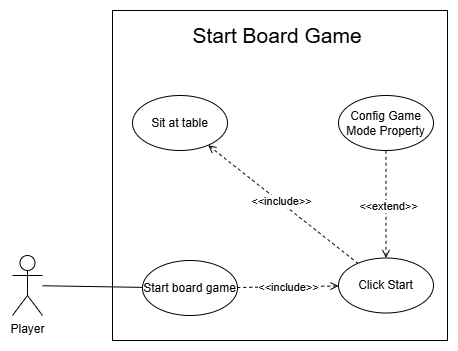
\includegraphics[width=0.75\linewidth]{4.Đặc tả chi tiết các lược đồ/Use-case/images/StartBoardGame.png}
    \caption{Use-case mô tả Start Board Game}
    \label{fig:placeholder}
\end{figure}


\begin{table}[H]
\centering
\begin{tabular}{|p{4cm}|p{10cm}|}
\hline
\textbf{Use-case name} & Start Board Game \\ \hline
\textbf{Actor} & Người chơi \\ \hline
\textbf{Descriptions} & Use-case này sẽ chỉ ra các bước cần thực hiện để có thể chơi được board game. \\ \hline
\textbf{Pre-conditions} & Phải vào được trong lobby \\ \hline
\textbf{Trigger} & Người chơi nhấn nút “Start” sau khi đã ngồi vào bàn và có từ 3 người chơi đang ngồi. \\ \hline
\textbf{Post-conditions} & Không có \\ \hline
\textbf{Normal Flow} &
\begin{enumerate}
\item Người chơi di chuyển đến ghế trống quanh bàn.
\item Người chơi nhấn giữ \textbf{''F''} để ngồi vào bàn.
\item Người chơi nhấn Start để bắt đầu vào game.
\end{enumerate}
\\ \hline
\textbf{Alternative Flow} &
\begin{enumerate}
\item[A1.] Trước bước 3, người chơi có thể chọn game mode và điều chỉnh thông số cần thiết của game mode đó.
\end{enumerate}
\\ \hline
\textbf{Exception Flow} &
\begin{enumerate}
\item[E1.] Tại bước 2, nếu bàn đang chơi thì không thể ngồi vào được
\item[E2.] Tại bước 3, nếu không đủ số người chơi đang ngồi thì không thể nhấn nút Start được.
\end{enumerate}
\\ \hline
\end{tabular}
\end{table}